\documentclass{beamer}
\usetheme{Boadilla}
\usepackage{essay-def}
\usepackage{bm}
\usepackage{amsfonts}
\usepackage{amssymb}
\usepackage{amsmath}
\usepackage{amsthm}
\usepackage{comment}
\usepackage{geometry}
\usepackage{enumerate}
\geometry{left=1cm,right=1cm}
    \title[NLG]{Natural language generation as dynamical systems}
\author[J. Zhao]{Jiaxi Zhao}
\date{13th May, 2024}
\begin{document}
\par \setlength{\parindent}{2em}
\newcommand{\JX}[1]{{\color{blue}{$^{\text{JX}}$[#1]}}}

\begin{frame}
\titlepage

\end{frame}

\begin{frame}{Language modeling}
	Language is very different from physics. Although humans began to study both at an early age, the theoretical foundations
	of language are far behind those of physics. Most successful approaches originate from the statistical modeling of the language, e.g.
	statistical learning and generative models etc.

	To model the language, the first task is to digitalize the text, which is made up of words, 
	into a sequence of numbers that can be manipulated by the computer.
\end{frame}

\begin{frame}{Word2Vec}
	Word2Vec\footnotemark[1] contains algorithms, e.g. continuous Bag-of-Words and continuous Skip-gram models 
	to learn the embedding vector of each word using corpus data. 

	vec(“Berlin”) - vec(“Germany”) + vec(“France”) = vec(“Paris”)

	vec(“Russian”) - vec(“River”) = vec(“Volga River”)
	\begin{figure}
		\centering
		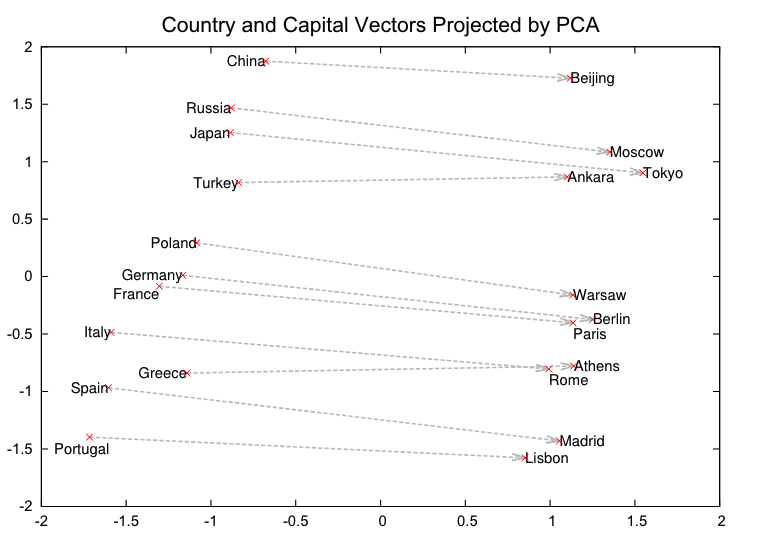
\includegraphics[width=0.4\textwidth]{fig/Word2Vec.jpg}
		\caption{Word2Vec: PCA from 1000D embedding to 2D}
	\end{figure}
	\footnotetext[1]{Distributed representations of words and phrases and their compositionality}
\end{frame}

\begin{frame}{Seq2Seq}
	Besides words and phrases, sentences can also have embeddings via the Seq2Seq framework:
	\begin{equation}
		\text{Input Seq} \overset{\text{Encoder}}{\Longrightarrow} \text{fixed-dim Vec} \overset{\text{Decoder}}{\Longrightarrow} \text{Output Seq}.
	\end{equation}
	\begin{figure}
		\centering
		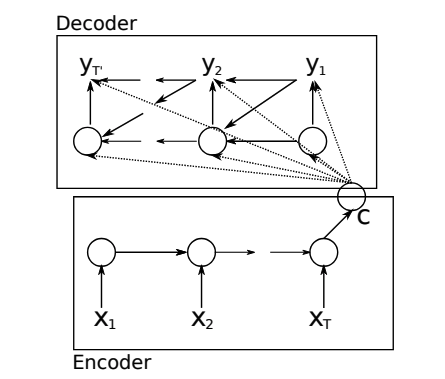
\includegraphics[width=0.4\textwidth]{fig/Seq2Seq_arch.jpg}
		\caption{Seq2Seq}
	\end{figure}
	\footnotetext[2]{Sequence to Sequence Learning with Neural Networks}
\end{frame}

\begin{frame}{Seq2Seq}
	Sentence embedding also has linguistic meaning:
	\begin{figure}
		\centering
		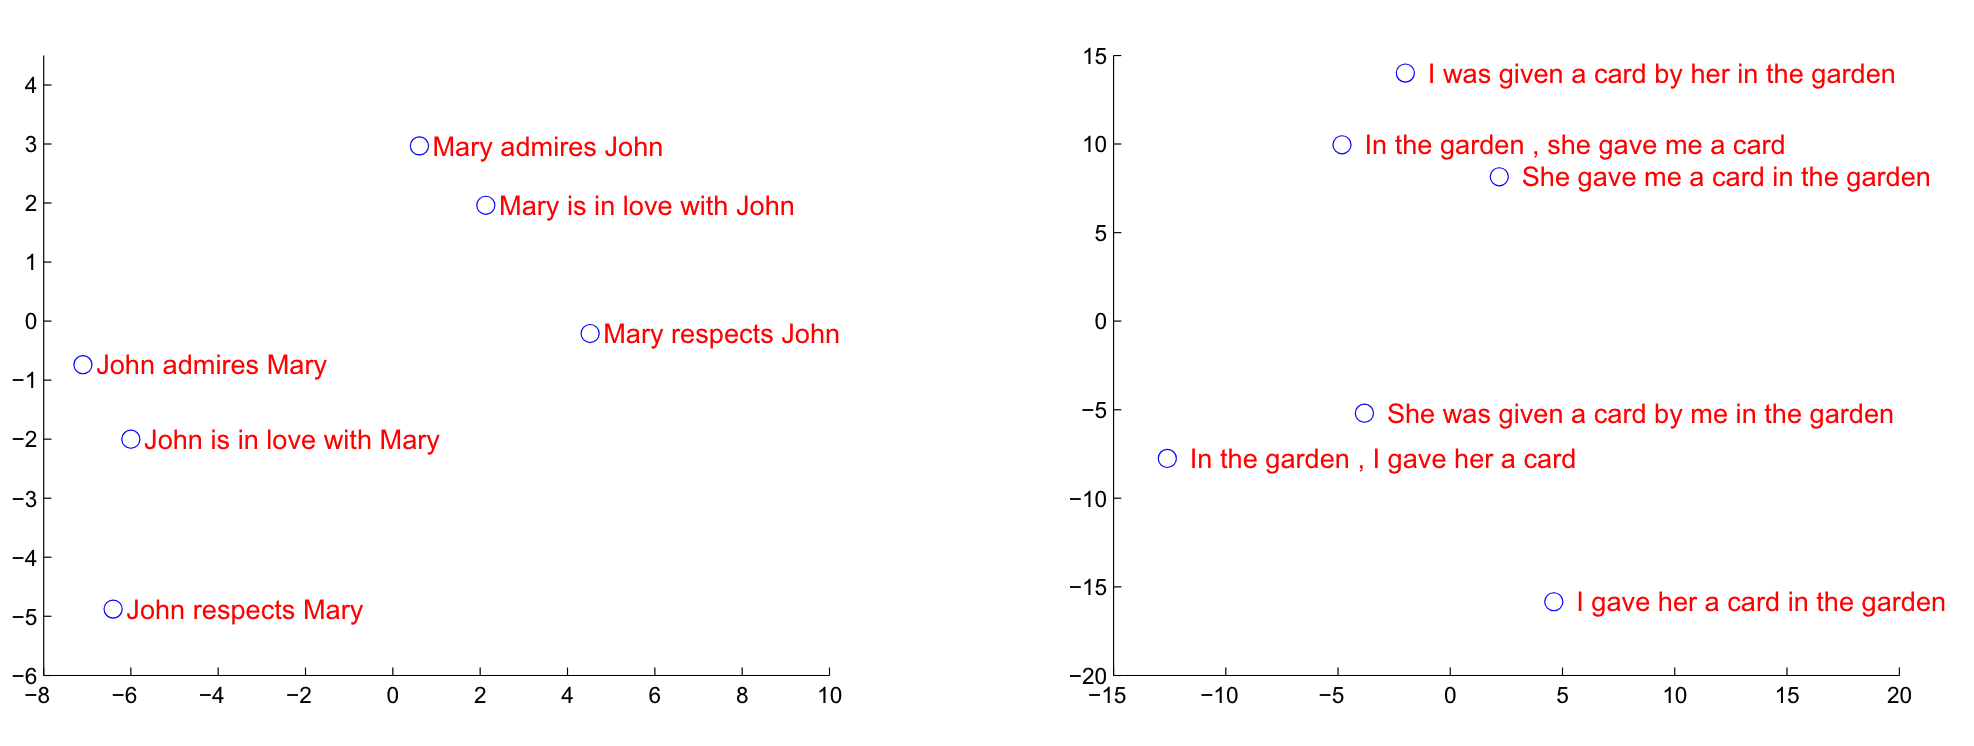
\includegraphics[width=\textwidth]{fig/Seq2Seq.jpg}
		\caption{Seq2Seq}
	\end{figure}
	\footnotetext[2]{Sequence to Sequence Learning with Neural Networks}
\end{frame}

\begin{frame}{Auto-regressive model: Tokenization \& embedding}
	The definition of natural language: \textit{Natural Language Generation, otherwise known as NLG, 
	is to produce natural written or spoken language from structured and unstructured data.}

	A step-by-step look at how LLMs generate a much longer sequence given a short prompt.
	\begin{equation}
		p(x_0, x_1, x_2, ..., x_T) = \prod_{t=1}^T p(x_t|x_{<t}).
	\end{equation}
	From text to a sequence of vectors:
	\begin{itemize}
		\item 1. Tokenization: The input text is tokenized into a sequence of tokens.
		\item 2. Word embedding: Each token is embedded into a high-dimensional vector space.
		\item 3. Positional encoding: The position of each token is encoded into the vector space.
	\end{itemize}
\end{frame}

\begin{frame}{Auto-regressive model: Attention}
	In self-attention, the query, key, and value are linear transformations of the input $X$:
	\begin{equation}
		Q = X W_Q, \quad K = XW_K, \quad V = XW_V.
	\end{equation}
	Notice that this calculation does not mix the vectors (tokens) at different positions. Then, a causal-masked
	attention is applied to obtain the attention matrix and output:
	\begin{equation}
		A(Q,K,V) = \text{softmax}(\frac{QK^T}{\sqrt{d_k}} \odot M)V.
	\end{equation}
	For multi-head attention, we split the query, key, and value into several small parts and 
	concatenate the outputs to obtain the final output
	\begin{equation}
		\begin{aligned}
			\text{MultiHead}(Q, K, V) & \ = \text{Concat}(\text{head}_1, ..., \text{head}_h)W^O,		\\
				\text{where } \ \text{head}_i & \ = A(QW_i^Q,KW_i^Q,VW_i^Q).
		\end{aligned}
	\end{equation}
	\footnotetext[3]{Attention is all you need}
\end{frame}

\begin{frame}{Auto-regressive model: Linear layer}
	An MLP is applied immediately after the attention layer to obtain the output:
	\begin{equation}
		FFN(x) = \max(0, xW_1 + b_1)W_2 + b_2.
	\end{equation}
	Similar to the query, key, and value projection, this calculation does not mix the vectors 
	(tokens) at different positions.
\end{frame}

\begin{frame}{Dynamics in the autoregressive model}
	There are at least two kinds of dynamics in the autoregressive model:
	\begin{itemize}
		\item The dynamics of the hidden states in the transformer, The dynamics of the hidden states in the 
		transformer architecture is intensively studied in the NLP literature \footnotemark[4].
		\item The dynamics of the autoregressive process.
	\end{itemize}
	However, as stated by Ilya Sutskever, the co-founder and chief scientist of OpenAI, \textbf{Next-token prediction
	is enough for AGI}. This dynamic is of great importance but not well understood.
	\footnotetext[4]{How Contextual are Contextualized Word Representations? Comparing the Geometry of BERT, ELMo, and GPT-2 Embeddings}
\end{frame}

\begin{frame}{Mistral 7B}
	We use Mistral 7B\footnotemark as the platform for our experiments, as it is reported to be the most powerful language 
	model for its size up to its release day (Sep 27, 2023). \textbf{You really should try it out!}

	\begin{itemize}
		\item Outperforms Llama 2 13B on all benchmarks
		\item Outperforms Llama 1 34B on many benchmarks
		\item Approaches CodeLlama 7B performance on code, while remaining good at English tasks
		\item Uses Grouped-query attention (GQA) for faster inference
		\item Uses Sliding Window Attention (SWA) to handle longer sequences at smaller cost
	\end{itemize}
	\footnotetext{https://arxiv.org/pdf/2310.06825, https://huggingface.co/mistralai/Mistral-7B-v0.1, 
	https://mistral.ai/news/announcing-mistral-7b/}
\end{frame}

\begin{frame}{Mistral 7B}
	\begin{figure}
		\centering
		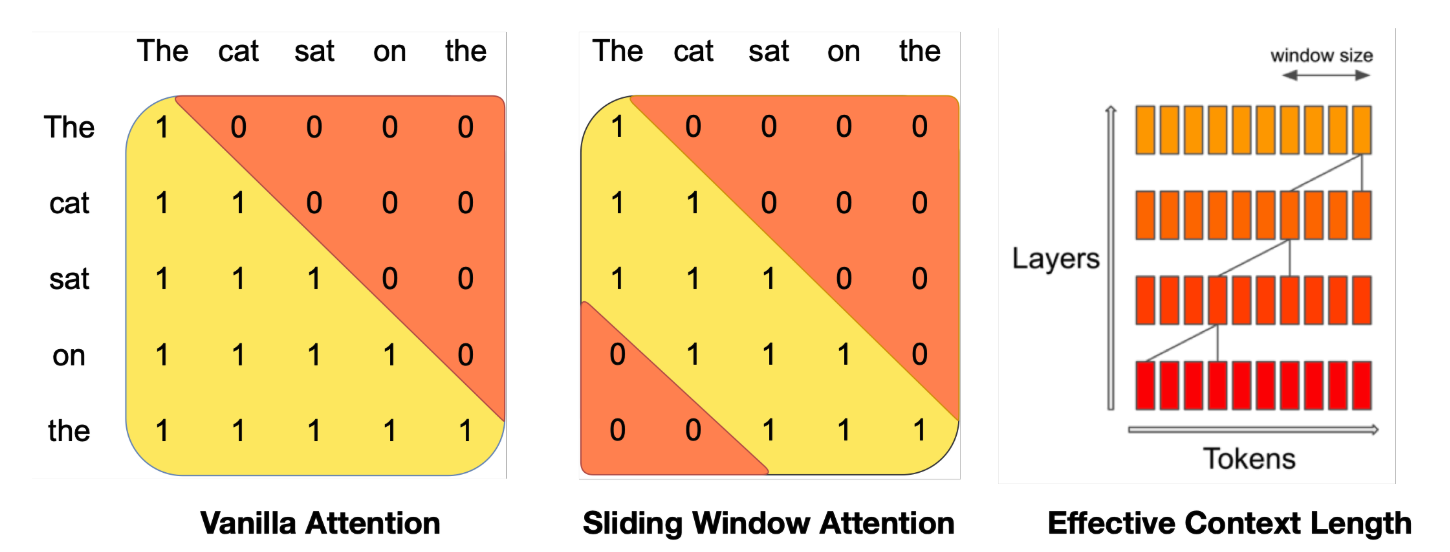
\includegraphics[width=0.8\textwidth]{fig/SWA.jpg}
		\caption{Sliding Window Attention}
	\end{figure}
	\begin{figure}
		\centering
		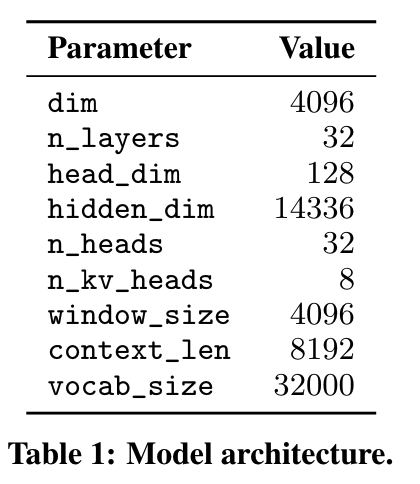
\includegraphics[width=0.4\textwidth]{fig/Mistral.jpg}
		\caption{Mistral hyperparameters}
	\end{figure}
\end{frame}

\begin{frame}{Decoding strategies}
	\begin{itemize}
		\item 1. Greedy decoding
		\begin{equation}
			x_t= \arg\max_{x} p(x_t|x_{<t}).
		\end{equation}
		\item 2. Beam search
		\item 3. Sampling: some out-lier word may spoil the NLG.
		\item 4. Top-k sampling: sampling from the first $k$ important tokens, no universal choice of $k$.
		\item 5. Top-p sampling: sampling from the first several important tokens which consist of $p$ of the probability mass.
	\end{itemize}
\end{frame}

\begin{frame}{Decoding strategies}
	\begin{figure}
		\centering
		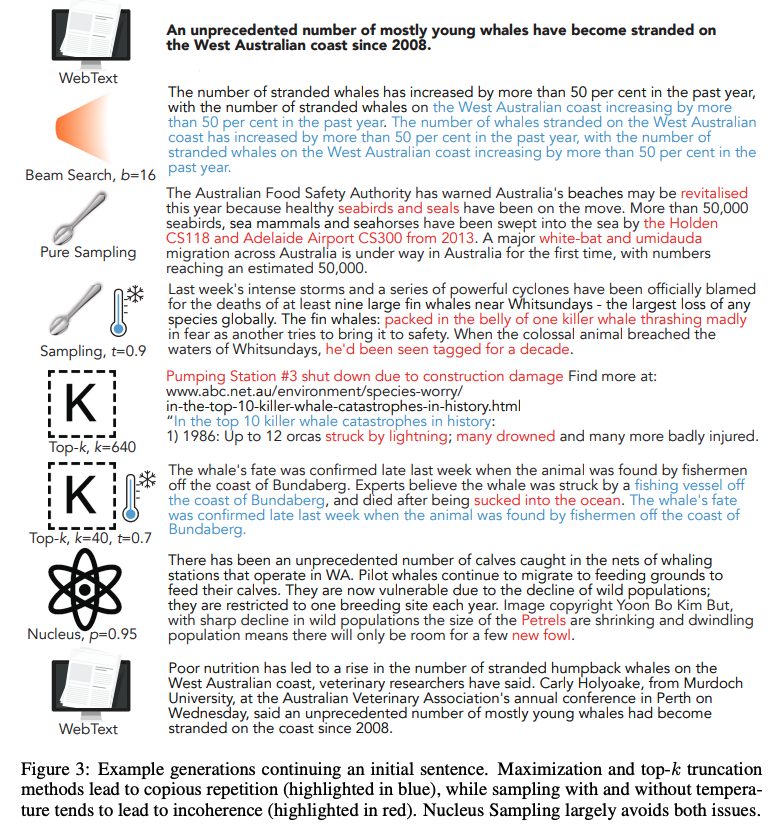
\includegraphics[width=0.8\textwidth]{fig/decoding.png}
		\caption{Word2Vec}
	\end{figure}
\end{frame}

\begin{frame}{Visualization of the word vector evolution}
	Using the prompt \textit{"Long time ago, there was a nymph,"}, we generate a sentence until EOS and visualize
	the sequences of word vectors over a low-dimensional space.
	\begin{figure}[ht]
		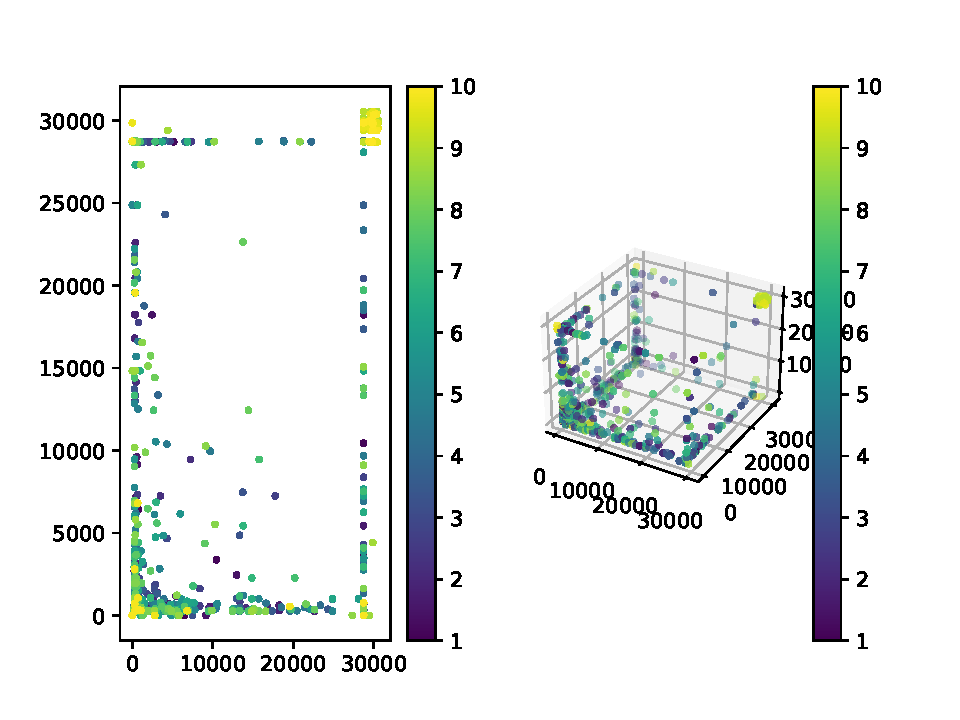
\includegraphics[width=.7\textwidth]{fig/delay_1.pdf}
		\caption{Delayed embedding}
	\end{figure}
\end{frame}

\begin{frame}{Visualization of the word vector evolution}
	\begin{figure}
		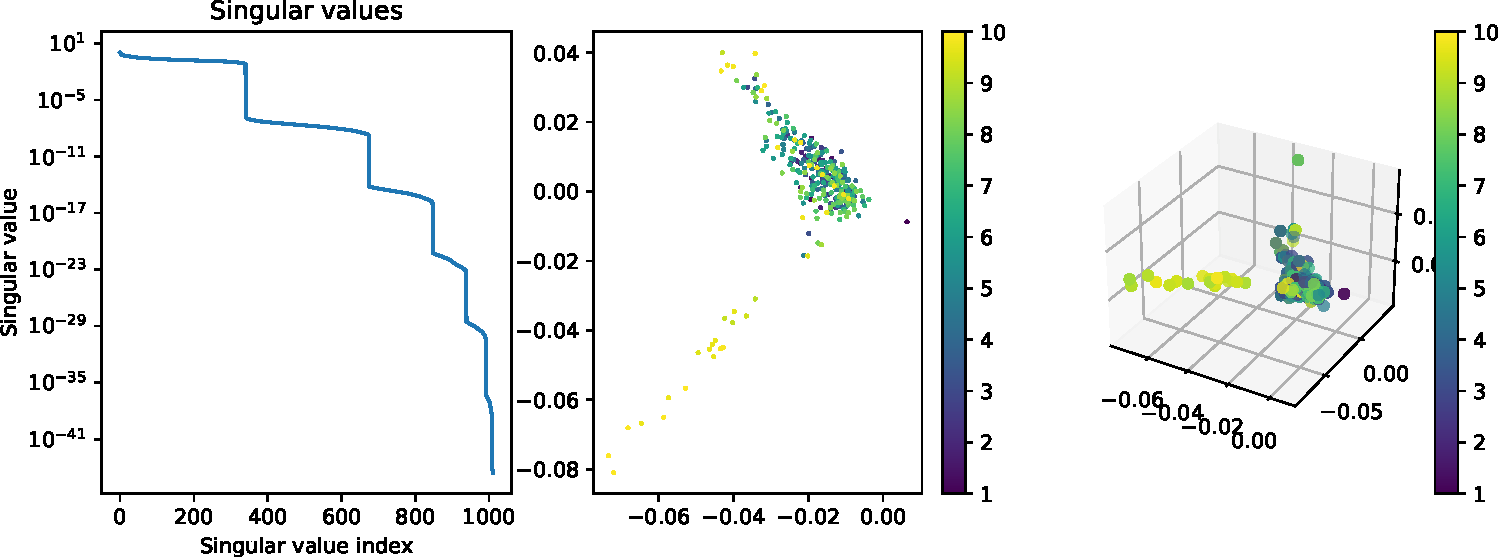
\includegraphics[width=\textwidth]{fig/pod_1.pdf}
		\caption{POD of word vector evolution}
	\end{figure}
\end{frame}

\begin{frame}{Visualization of the probability evolution}
	The well-known Zipf law states that the frequency of a word is inversely proportional to its rank in the frequency table
	\begin{equation}
		P(X=k) \propto \frac{1}{k^{\alpha}}.
	\end{equation}
	\begin{figure}[ht]
		\centering
		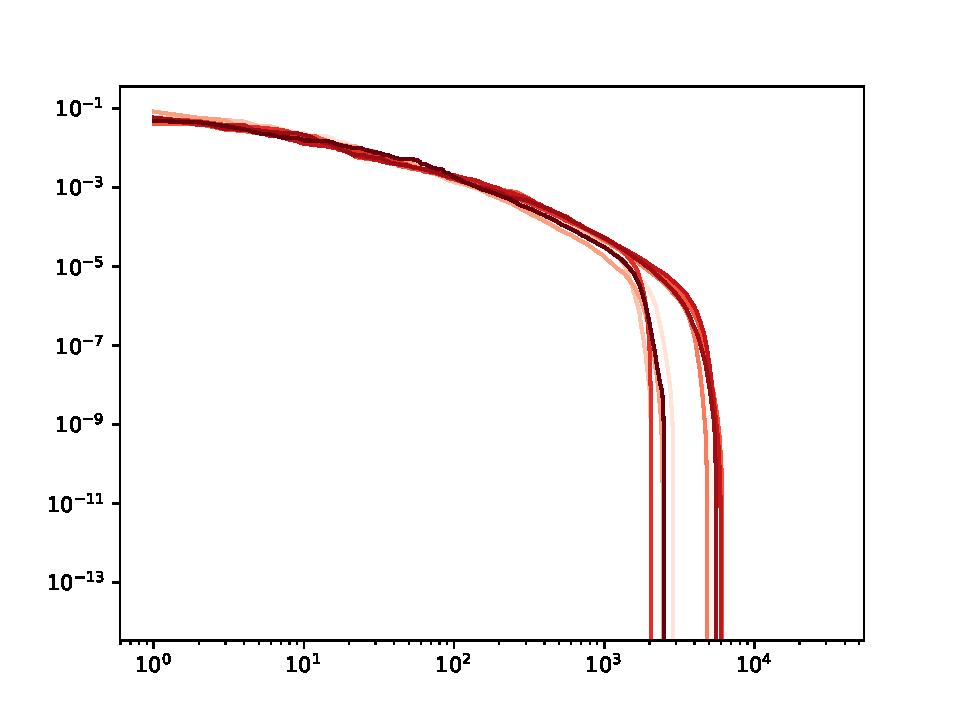
\includegraphics[width=.7\textwidth]{fig/zipf.pdf}
		\caption{Comparison with Zipf law}
	\end{figure}
\end{frame}

\begin{frame}{Visualization of the probability evolution}
	Similar to the idea of Word2Vec, we would like to use this distribution to perform clustering on the
	vocabulary, which implies their dynamic correlation in NLG. Namely, the probability distribution of shape
	[vocab size, seq length] can be viewed as another embedding of the word to high-dimensional space
\end{frame}

\begin{frame}{Visualization of the probability evolution}
	From the other perspective, we can also perform dimension reduction over the vocab\_size dimension
	to visualize the dynamic of the probability evolution:
	\begin{figure}[ht]
		\centering
		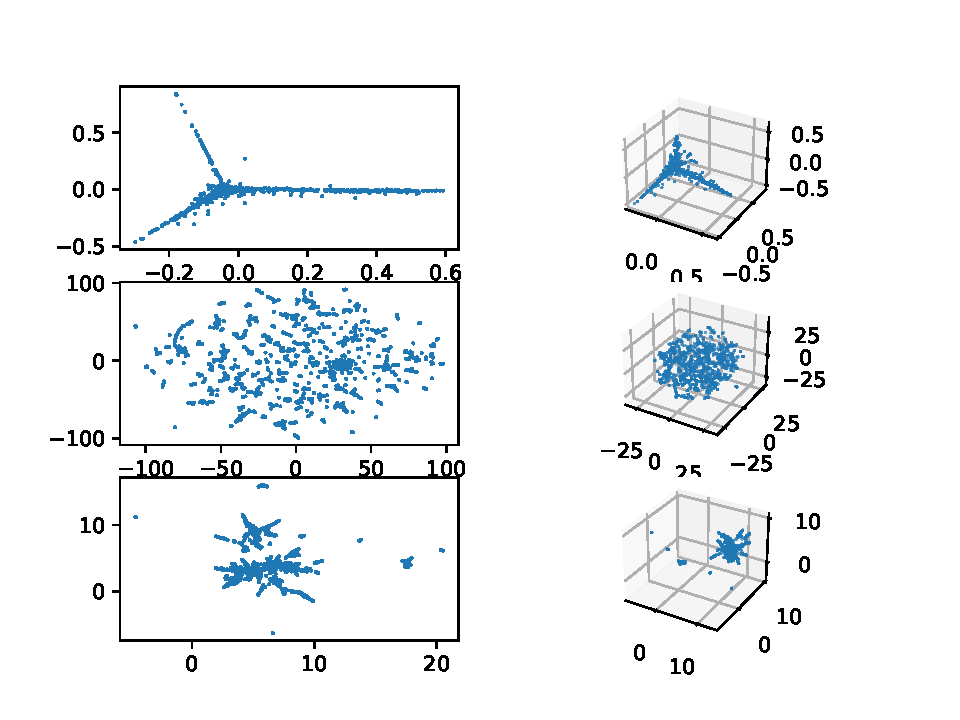
\includegraphics[width=.7\textwidth]{fig/prob_evolve_0.pdf}
		\caption{Low-dim visualization of the distribution evolution}
	\end{figure}
\end{frame}

\begin{frame}{Visualization of the probability evolution}
	More interesting patterns
	\begin{figure}[ht]
		\centering
		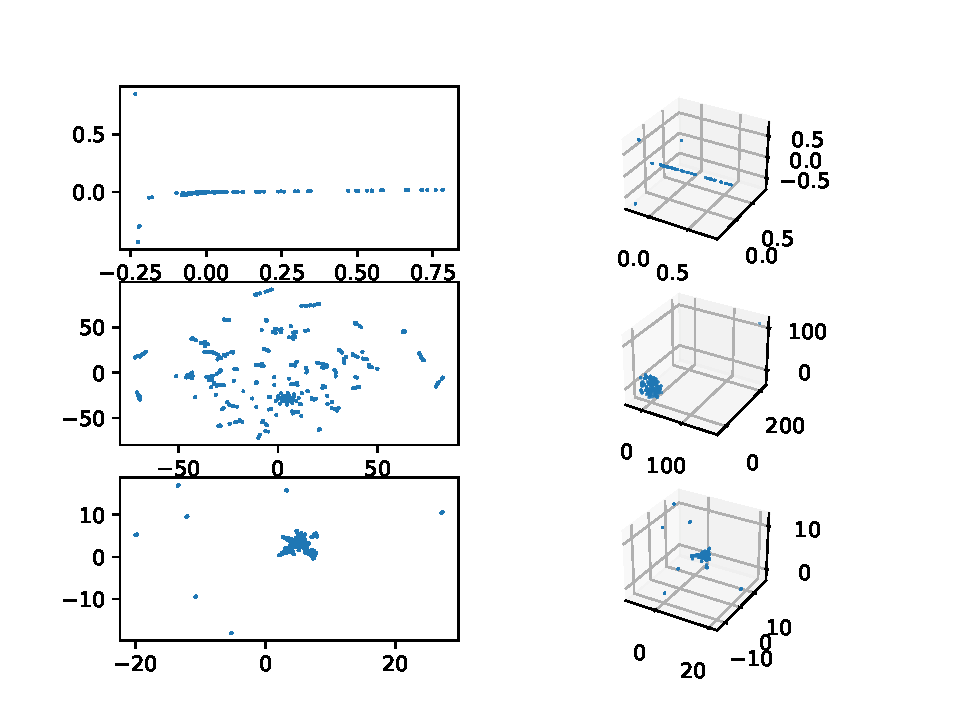
\includegraphics[width=\textwidth]{fig/prob_evolve_1.pdf}
		\caption{Low-dim visualization of the distribution evolution}
	\end{figure}
\end{frame}

\begin{frame}{Visualization of the probability evolution}
	More interesting patterns
	\begin{figure}[ht]
		\centering
		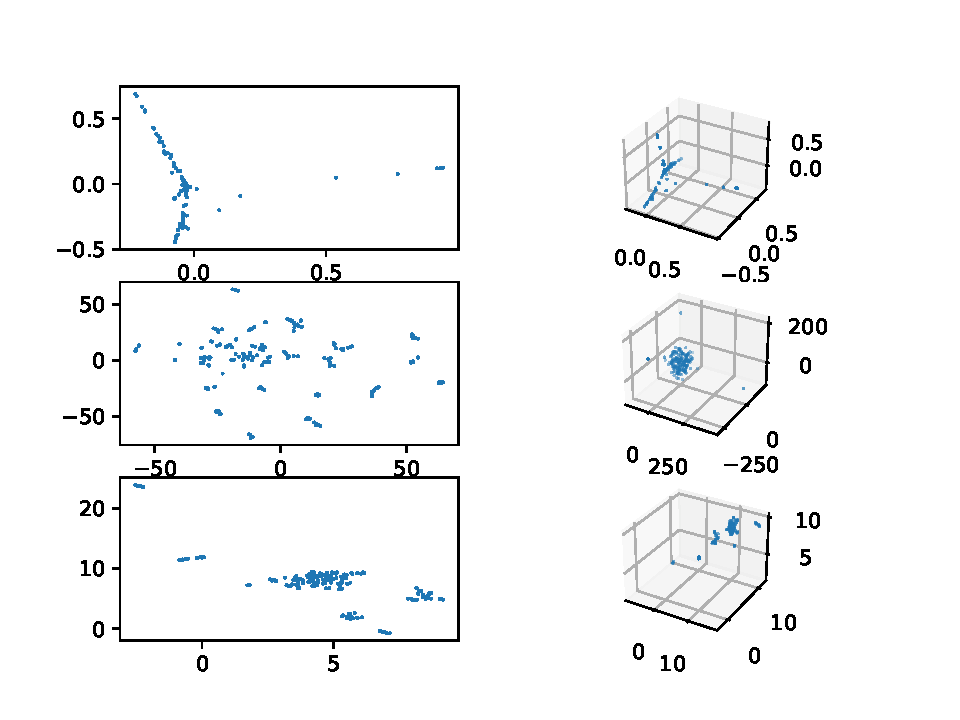
\includegraphics[width=\textwidth]{fig/prob_evolve_2.pdf}
		\caption{Low-dim visualization of the distribution evolution}
	\end{figure}
\end{frame}

\begin{frame}{State variable of the NLG}
	Key question: \textit{Viewing the NLG as a dynamical system, what is the state variable of it?}

	We need some quantities that are informative enough to encode the whole information in a forward pass 
	of the LLMs. Here are some obvious choices:
	\begin{itemize}
		\item 1. Zero padding for shorter sequences at the beginning and use the maximum length as the fixed
		dimension hidden state (usually 4k, even 32k). \JX{Markovian model reduction}
		\item 2. Use the attention matrices of all heads or their spectral information.
		\item 3. In Seq2Seq, the hidden state of the encoder can be used as the state variable. But decoder-only 
		autoregressive models like GPT do not belong to the Seq2Seq category(personal idea), do they?
		\item 4. \JX{This may be a non-Markov model, need to use another definition of chaoticity.}
	\end{itemize}
\end{frame}

\begin{frame}{Future directions}
	Further questions:
	\begin{itemize}
		\item 1. How does prompt engineering change the dynamics of the NLG in LLMs?
		\JX{This seems to be an interesting direction. But the prompt engineering is far from choosing the initial condition, 
		it is more like choosing the boundary so that the generator will not go out of this boundary.}
		\item 2. Can we use the tools from information theory such as minimal description length to understand the
		the dynamics of the NLG?
		\item 3. Investigate the dynamics of the autoregressive process in the LLMs for different contexts, e.g. novel, academic journal, and code etc.
		Ablation studies on different LLMs and different scales should also be explored.
		\item 4. What's more?
	\end{itemize}
\end{frame}

\begin{frame}{Reference}
	\begin{itemize}
		\item 1. Mikolov, Tomas, et al. "Distributed representations of words and phrases and their compositionality." Advances in neural information processing systems 26 (2013).
		\item 2. Sutskever, Ilya, Oriol Vinyals, and Quoc V. Le. "Sequence to sequence learning with neural networks." Advances in neural information processing systems 27 (2014).
		\item 3. Vaswani, Ashish, et al. "Attention is all you need." Advances in neural information processing s
		\item 4. Jiang, Albert Q., et al. "Mistral 7B." arXiv preprint arXiv:2310.06825 (2023).
	\end{itemize}
\end{frame}

\begin{frame}{Reference}
	\begin{itemize}
		\item 5. How Contextual are Contextualized Word Representations? Comparing the Geometry of BERT, ELMo, and GPT-2 Embeddings (Ethayarajh, EMNLP-IJCNLP 2019)
		\item 6. Holtzman, Ari, et al. "The curious case of neural text degeneration." arXiv preprint arXiv:1904.09751 (2019).
	\end{itemize}
\end{frame}

\end{document}